% !Mode:: "TeX:UTF-8"
% !TEX program  = xelatex
\title{Assignment 7}


\section{Question 1}
\begin{statebox}{Timescale Invariance}{question-1}
    \begin{align*}
        d_1 &= \frac{\log(S/E)+(r+\sigma^2/2)(T-t)}{\sigma\sqrt{T-t}} \\
        d_1 &= \frac{\log(S/E)+(r-\sigma^2/2)(T-t)}{\sigma\sqrt{T-t}}
    \end{align*}
    Prove the following identity:
    \[
    	d_2 = d_1 - \sigma\sqrt{T-t}
    \]
\end{statebox}

\Python{}{code/7-a.py}



\section{Question 2}
\begin{statebox}{Put-Call Parity}{question-2}
    With $t=0$, $S_0=5$, $E=4$, $T=1$, $\sigma=0.3$ and $r=0.05$, find the option values and verify the put-call parity.
\end{statebox}

\Python{}{code/7-b.py}



\section{Question 3}
\begin{statebox}{Study Note}{question-3}
    \begin{enumerate}
    	\item Write a study note of Black-Scholes' 73 paper.
    	\item Find a sequence of works following this paper and sort out hot topics nowadays.
    \end{enumerate}
\end{statebox}

\subsection{The Black-Scholes World}
The Black–Scholes model assumes that the market consists of at least one risky asset, usually called the stock, and one riskless asset, usually called the money market, cash, or bond. Now we make assumptions on the assets (which explain their names):
\begin{itemize}
    \item (riskless rate) The rate of return on the riskless asset is constant and thus called the \href{https://en.wikipedia.org/wiki/Risk-free_interest_rate}{risk-free interest rate}.
    \item (random walk) The instantaneous log return of stock price is an infinitesimal \href{https://en.wikipedia.org/wiki/Random_walk}{random walk} with drift; more precisely, the stock price follows a \href{https://en.wikipedia.org/wiki/Geometric_Brownian_motion}{geometric Brownian motion}, and we will assume its drift and volatility are constant (if they are time-varying, we can deduce a suitably modified Black–Scholes formula quite simply, as long as the volatility is not random).
    \item The stock does not pay a \href{https://en.wikipedia.org/wiki/Dividend}{dividend}.
\end{itemize}

Assumptions on the market:
\begin{itemize}
    \item There is no \href{https://en.wikipedia.org/wiki/Arbitrage}{arbitrage} opportunity (i.e., there is no way to make a riskless profit).
    \item It is possible to borrow and lend any amount, even fractional, of cash at the riskless rate.
    \item It is possible to buy and sell any amount, even fractional, of the stock (this includes \href{https://en.wikipedia.org/wiki/Short_selling}{short selling}).
    \item The above transactions do not incur any fees or costs (i.e., \href{https://en.wikipedia.org/wiki/Frictionless_market}{frictionless market}).
\end{itemize}


\subsection{Black–Scholes Equation}
As above, the \textbf{Black–Scholes equation} is a \href{https://en.wikipedia.org/wiki/Partial_differential_equation}{partial differential equation}, which describes the price of the option over time. The equation is:
\begin{equation}\label{F:black-scholes}
    \frac{\partial V}{\partial t} + \frac{1}{2}\sigma^2S^2\frac{\partial^2V}{\partial S^2} + rS\frac{\partial V}{\partial S} - rV = 0.
\end{equation}


\subsection{Black–Scholes Formula}
The value of a call option for a non-dividend-paying underlying stock in terms of the Black–Scholes parameters is:
\begin{equation}\label{F:black-scholes-2}
    \begin{aligned}
        C(S_t,t) &= N(d_1)S_t - N(d_2)PV(K) \\
        d_1 &= \frac{1}{\sigma\sqrt{T-t}}\left[\ln\left(\frac{S_t}{K}\right)+\left(r+\frac{\sigma^2}{2}\right)(T-t)\right] \\
        d_2 &= d_1 - \sigma\sqrt{T-t} \\
        PV(K) &= K\exp{(-r(T-t))}
    \end{aligned}
\end{equation}

The price of a corresponding put option based on put–call parity is:
\begin{equation}\label{F:black-scholes-3}
    \begin{aligned}
        P(S_t,t) &= K\exp{(-r(T-t))} - S_t + C(S_t,t) \\
        &= N(-d_2)K\exp{(-r(T-t))} - N(-d_1)S_t.
    \end{aligned}
\end{equation}
\begin{figure}[H]
    \centering
    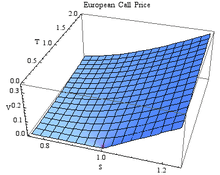
\includegraphics[width=.5\textwidth]{figures/2019-11-13-black-scholes-6}
    \caption{A European call valued using the Black-Scholes pricing equation for varying asset price $S$ and time-to-expiry $T$}\label{F:black-scholes-6}
\end{figure}



\begin{figure}[H]
    \centering
    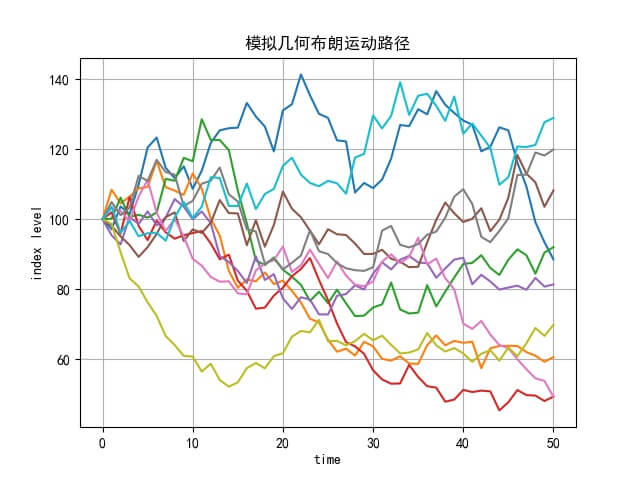
\includegraphics[width=.7\textwidth]{figures/2019-11-13-black-scholes-1}
    \caption{Simulated geometric Brownian motions with parameters from market data}\label{F:black-scholes-1}
\end{figure}

\begin{figure}[H]
    \centering
    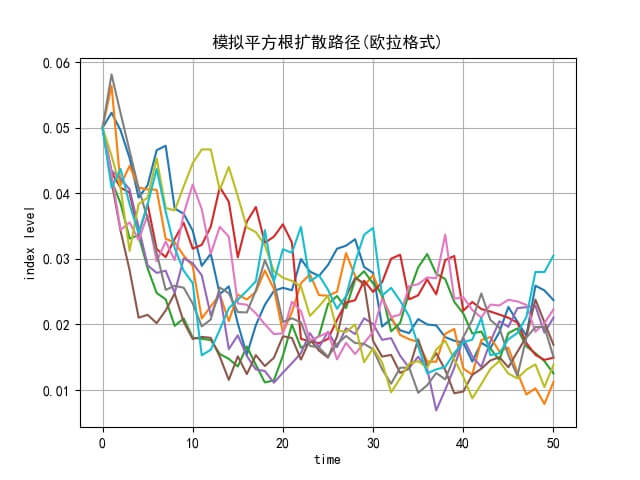
\includegraphics[width=.7\textwidth]{figures/2019-11-13-black-scholes-2}
\end{figure}

\begin{figure}[H]
    \centering
    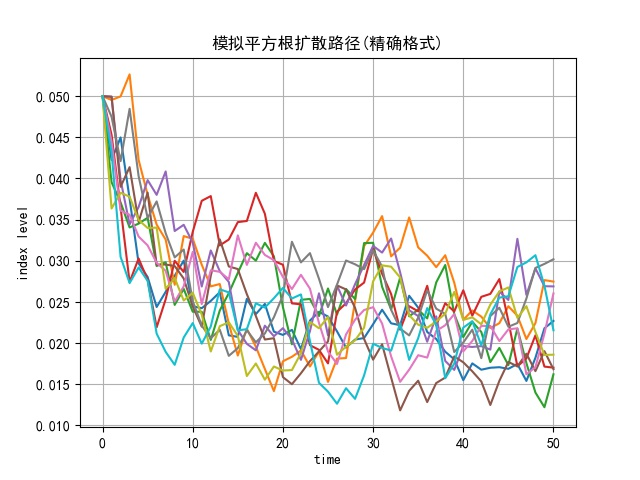
\includegraphics[width=.7\textwidth]{figures/2019-11-13-black-scholes-3}
\end{figure}

\begin{figure}[H]
    \centering
    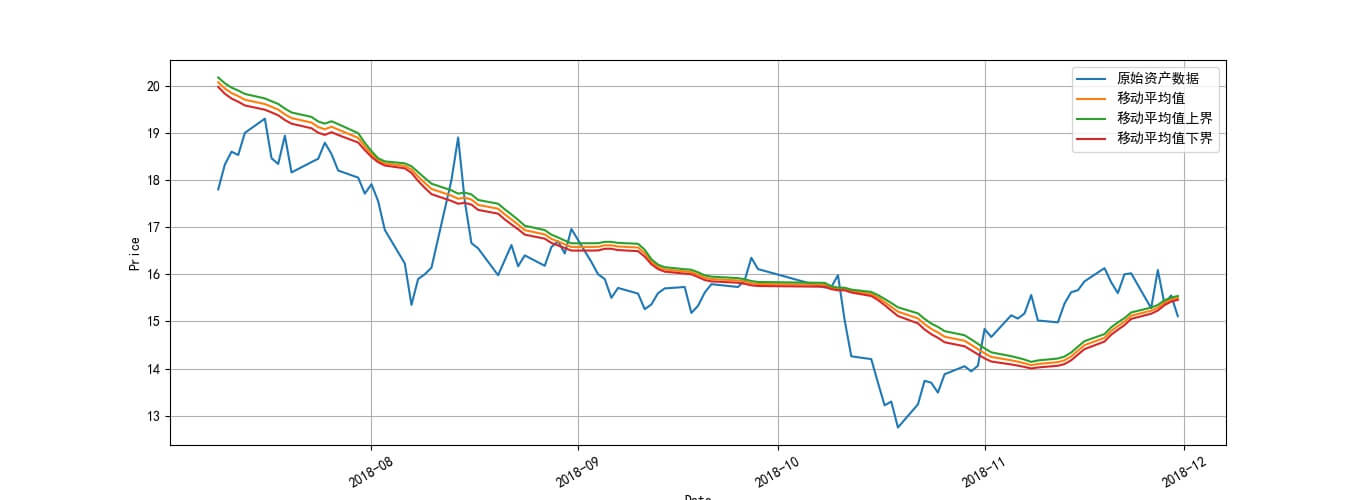
\includegraphics[width=\textwidth]{figures/2019-11-13-black-scholes-4}
    \caption{Bolling graph}\label{F:black-scholes-4}
\end{figure}

\begin{figure}[H]
    \centering
    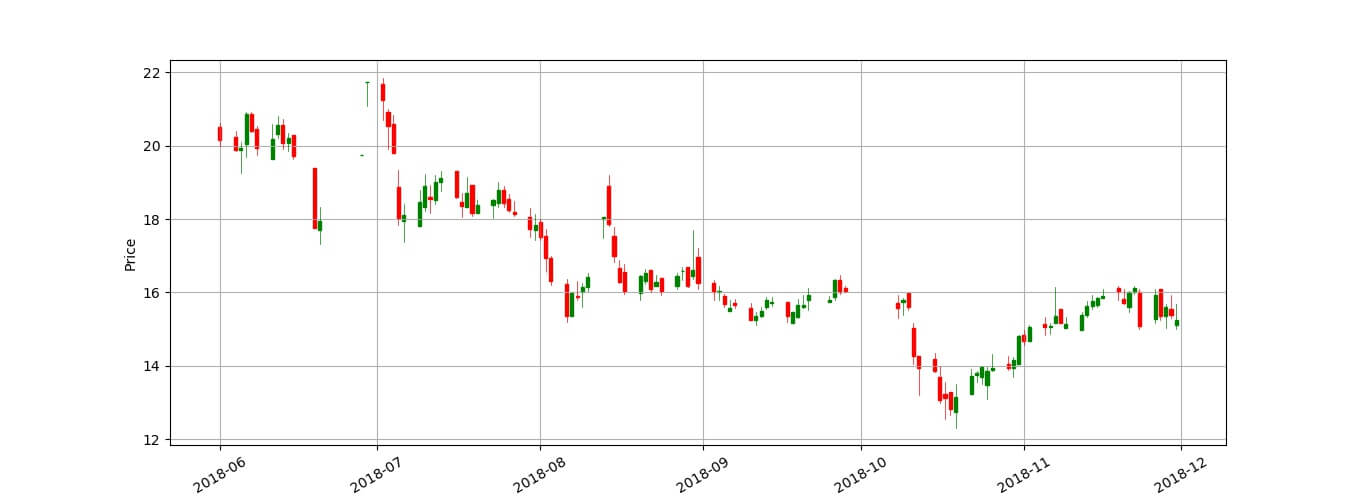
\includegraphics[width=\textwidth]{figures/2019-11-13-black-scholes-5}
    \caption{Candle graph}\label{F:black-scholes-5}
\end{figure}



\appendix
    \section{Simulation Program}
        \Python{simulation.py}{code/simulation.py}
    \section{Plot Function}
        \Python{bolling.py}{code/plot/bolling.py}
        \Python{candle.py}{code/plot/candle.py}
